% Files using this must be two subfolders
% deep. Adjust the number of ../ for the
% depth of the file.
% Imports
\usepackage{fancyhdr}
\usepackage{geometry}
\usepackage{icomma}
\usepackage{amsmath}
\usepackage{multicol}
\usepackage{mathptmx}
\usepackage{anyfontsize}
\usepackage{t1enc}
\usepackage{tabto}
\usepackage{listings}
\usepackage{filecontents}
\usepackage{subcaption}
\usepackage{tikz}
\usepackage[parfill]{parskip}
\usepackage{graphicx}
\usepackage[]{mdframed}
\usepackage{amsmath}
\usepackage[makeroom]{cancel}
\usepackage{pgfplots}
\usepackage{pgfplotstable}
\usepackage{xfrac}
\usepackage{amssymb}
\usepackage{mathtools}
\pgfplotsset{compat=1.18}
\usetikzlibrary{patterns}
\usepgfplotslibrary{polar}
\usepgfplotslibrary{fillbetween}

\geometry{margin=2.5cm}

\newcommand{\name}{Kaleb Burris}
\newcommand{\classname}{MATH F253, Elizabeth S. Allman, University of Alaska Fairbanks}
\newcommand{\assignment}{FILL IN ASSIGNMENT NAME}

\pagestyle{fancy}

\fancyhead[L]{
    \name 
    \newline
    \classname
    \newline
    \assignment
}

\newcommand{\horizontal}{\noindent\rule{\hsize}{0.4pt}}

\setlength{\headheight}{42pt}
\setlength{\headsep}{0.25in}
\setlength{\columnsep}{0.35cm}
\setlength{\columnseprule}{1pt}

\usepackage[T1]{fontenc}
\usepackage{lmodern}

\usepackage{enumitem}
\usepackage{graphicx}
\graphicspath{ {./lab05images/} }

% Put class number, class name, and professor 
% name.
% Use only in case of emergency, this
% should be covered by the preamble.
% \renewcommand\classname{}

% Put the assignment name with \S if 
% necessary for the section and the question 
% numbers.
\renewcommand\assignment{Lab 5: Conservation of Mechanical Energy , 2/28/2023, Partners: Maite Valentin-Lugo, Seth Waln}

\begin{document}

    % Templates
    \iffalse
    % Use these for equations.
    \begin{equation*}
        \begin{gathered}
            Equations go here.
        \end{gathered}
    \end{equation*}

    % Use this if a line of math is too long.
    \resizebox{\hsize}{!}{$Long equation goes here$}

    % Use these for multiple columns.
    \begin{multicol*}{# of columns}
        % Remove the * if you want the columns to be balanced.
    \end{multicol*}

    % Use this to add a horizontal line.
    \horizontal

    \fi

    % Begin homework here.
    %%%%%%%%%%%%%%%%%%%%%%

    I was pretty sick when I filled in this lab. Forgive the terrible formatting and cheapskate images.

    \paragraph*{1.}

    \begin{equation*}
        E = K + U
    \end{equation*}

    Mechanical energy is the sum of the kinetic and potential energy in a system, so changing one will have a linear effect on the other.

    \begin{equation*}
        U = \frac{1}{2}(k_{1})(x-x_{e})^{2} + U_{0}
    \end{equation*}

    For springs, the potential energy is half of the spring constant times the displacement squared plus any initial potential energy.

    \begin{equation*}
        K = \frac{1}{2}\left[M + \frac{1}{3}(m_{1} + m_{2})\right]v^{2}
    \end{equation*}

    Kinetic energy is based on the mass of the system and the velocity squared.

    \paragraph*{2.}\hbox{}

    Force = mx+b

    m (Slope): -7.965 N/m

    b (Y-Intercept): 7.591 N

    Correlation: -0.6982

    RMSE: 0.07085 N

    \paragraph*{3.}\hbox{}

    RMSE: 0.07085 N

    \paragraph*{4.}\hbox{}

    The spring constant is the negative of the slope (from question 2).
 	$k$ = 7.965 N/m

    \paragraph*{5., 6.}\hbox{}

    \begin{center}
        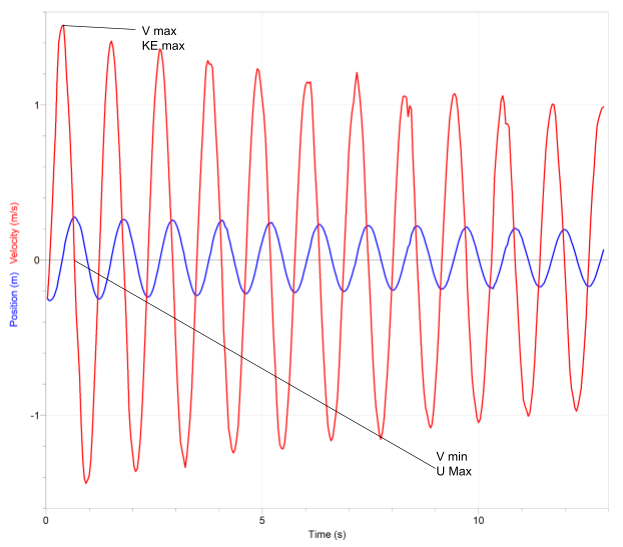
\includegraphics[width=0.5\textwidth]{image20.png}
    \end{center}

    \paragraph*{7.}\hbox{}

    \begin{center}
        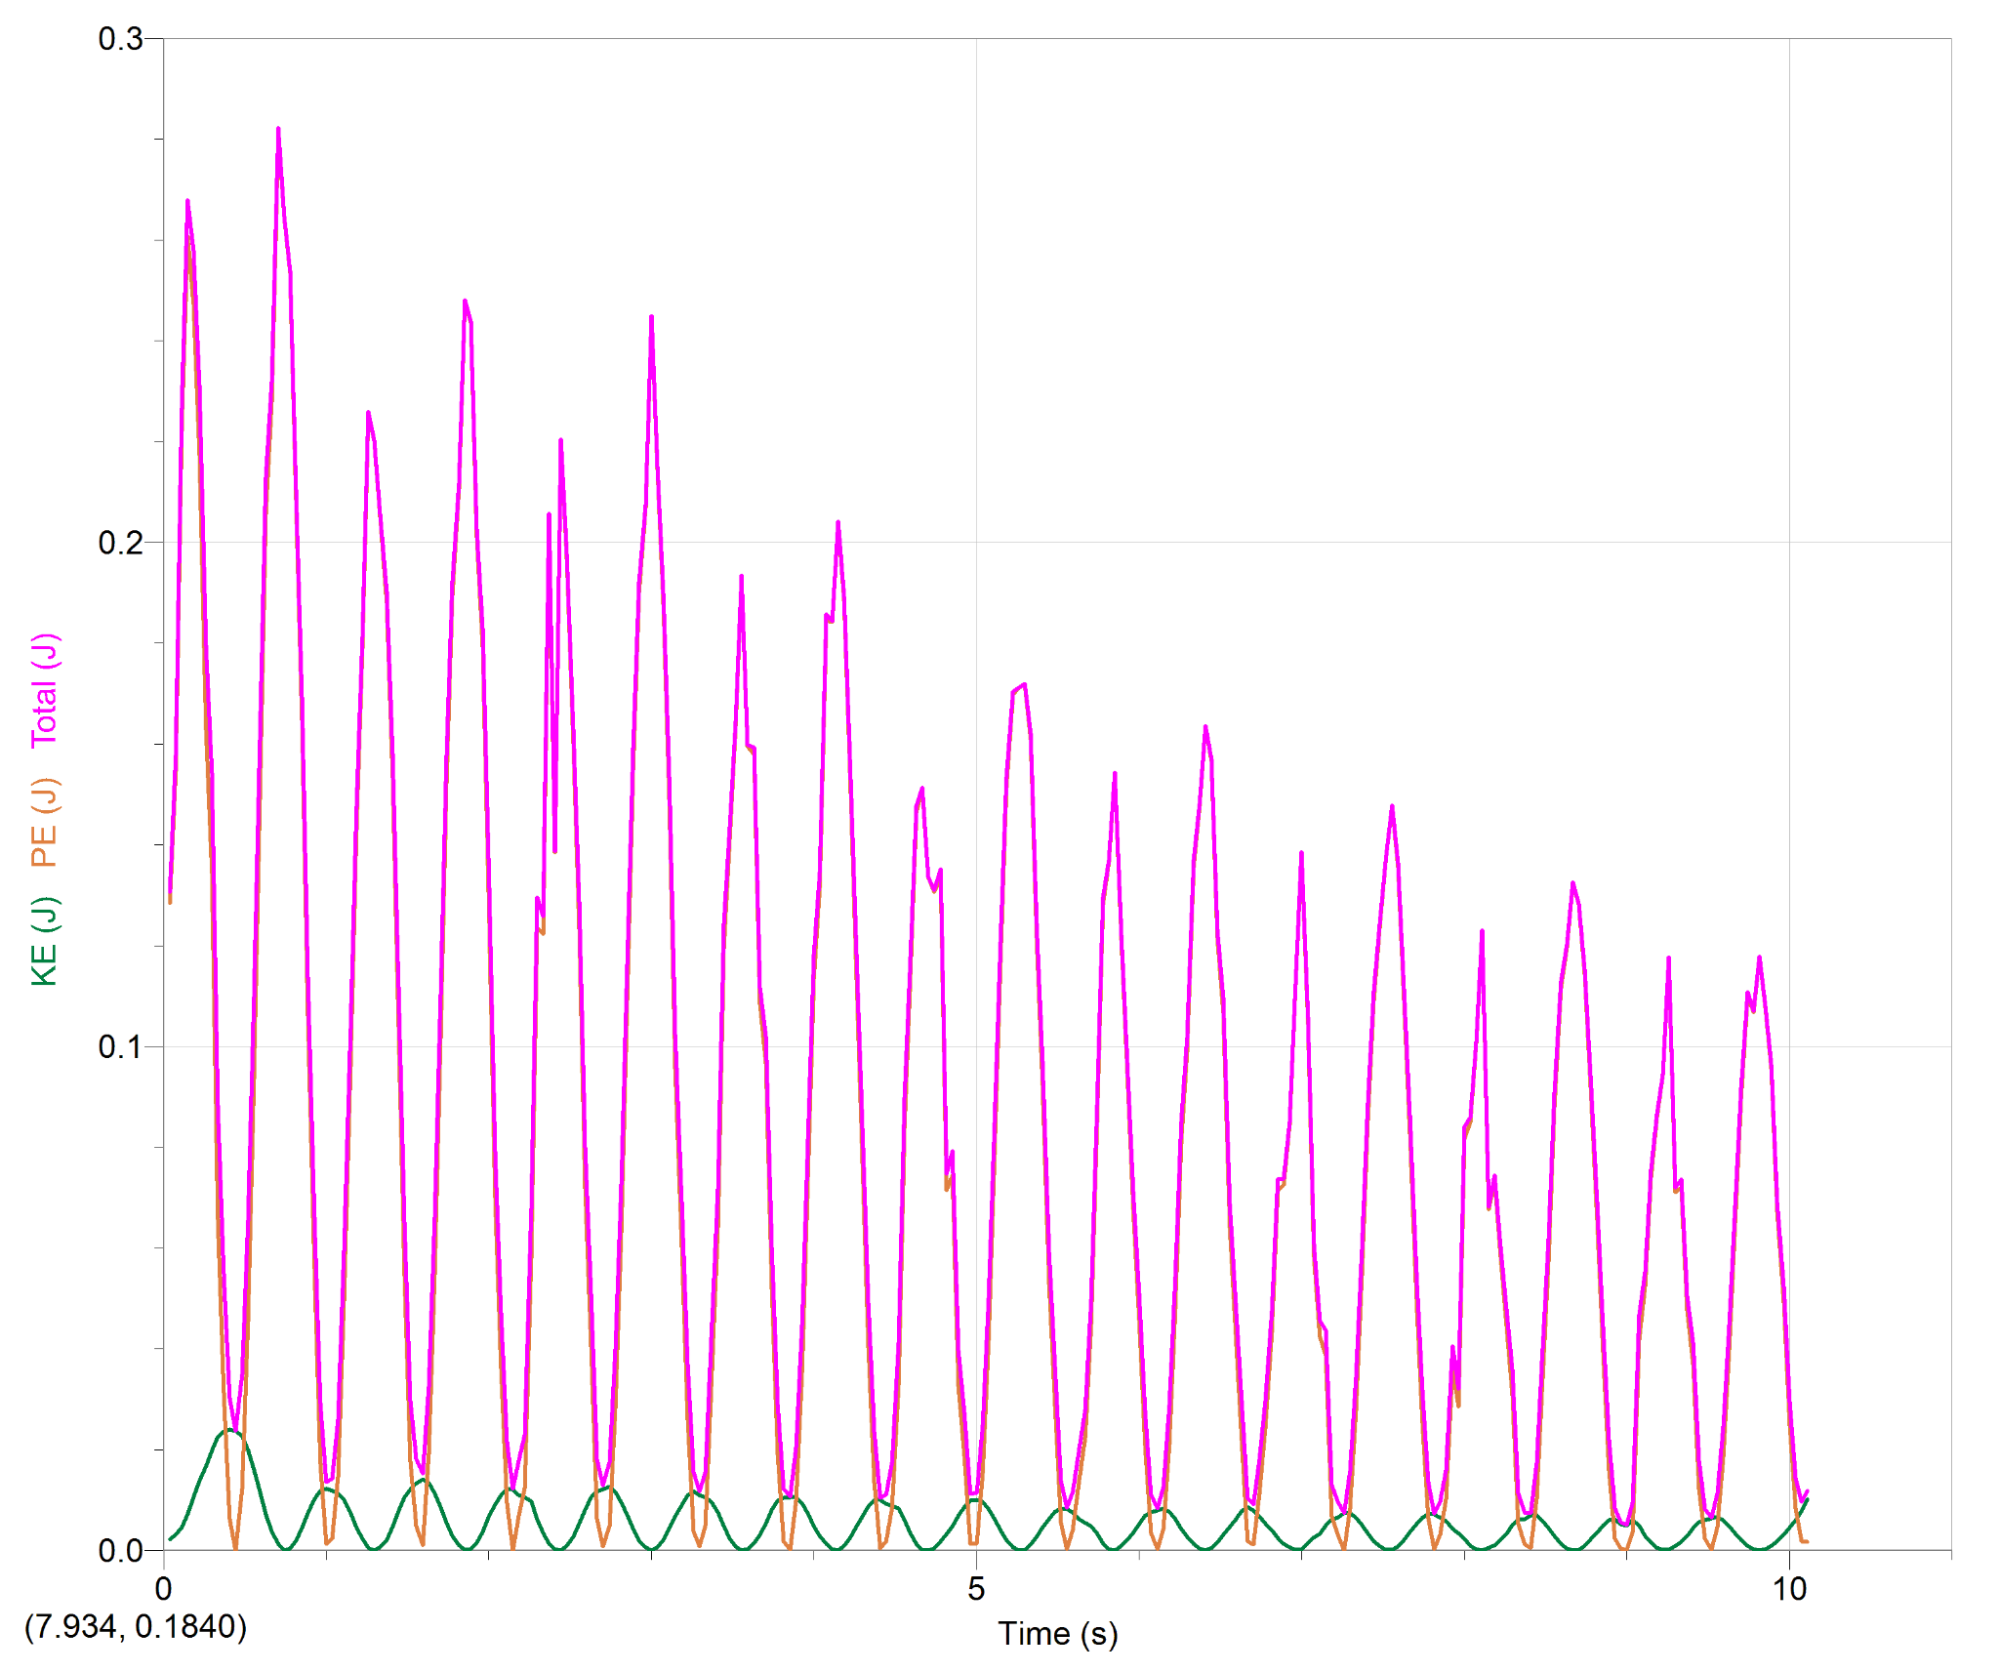
\includegraphics[width=0.5\textwidth]{image21.png}
    \end{center}

    \paragraph*{8.}\hbox{}
    
    Manual Fit for: Latest | Total 
    E = A*exp(-C*t)+B
    A: 0.1575
    C: 0.09993
    B: 0.009152

    A is the initial energy 

    B is final energy in the system

    C is energy loss due to friction

    \paragraph*{9.}

    Logger pro says the RMSE  is $\pm$ 0.07085 N. Given just how shaky my hands were, this uncertainty seems pretty low, although the algorithm for RMSE is relatively good at filtering outliers. 

    \paragraph*{10.}

    Linear Fit for: Latest | Force 

    Force = mx+b

    m (Slope): -7.582 N/m

    b (Y-Intercept): -0.05095 N

    Correlation: -0.9978

    RMSE: 0.05060 N

    Linear Fit for: Latest | Force 
    
    Force = mx+b

    m (Slope): -7.850 N/m

    b (Y-Intercept): -0.1560 N

    Correlation: -0.9969

    RMSE: 0.06398 N

    Average relative uncertainty = $\boxed{0.00742}$

    \pagebreak

    \paragraph*{11.}

    \begin{center}
        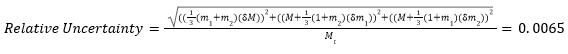
\includegraphics[width=0.8\textwidth]{image50.png}
    \end{center}

    \paragraph*{12.}

    \begin{center}
        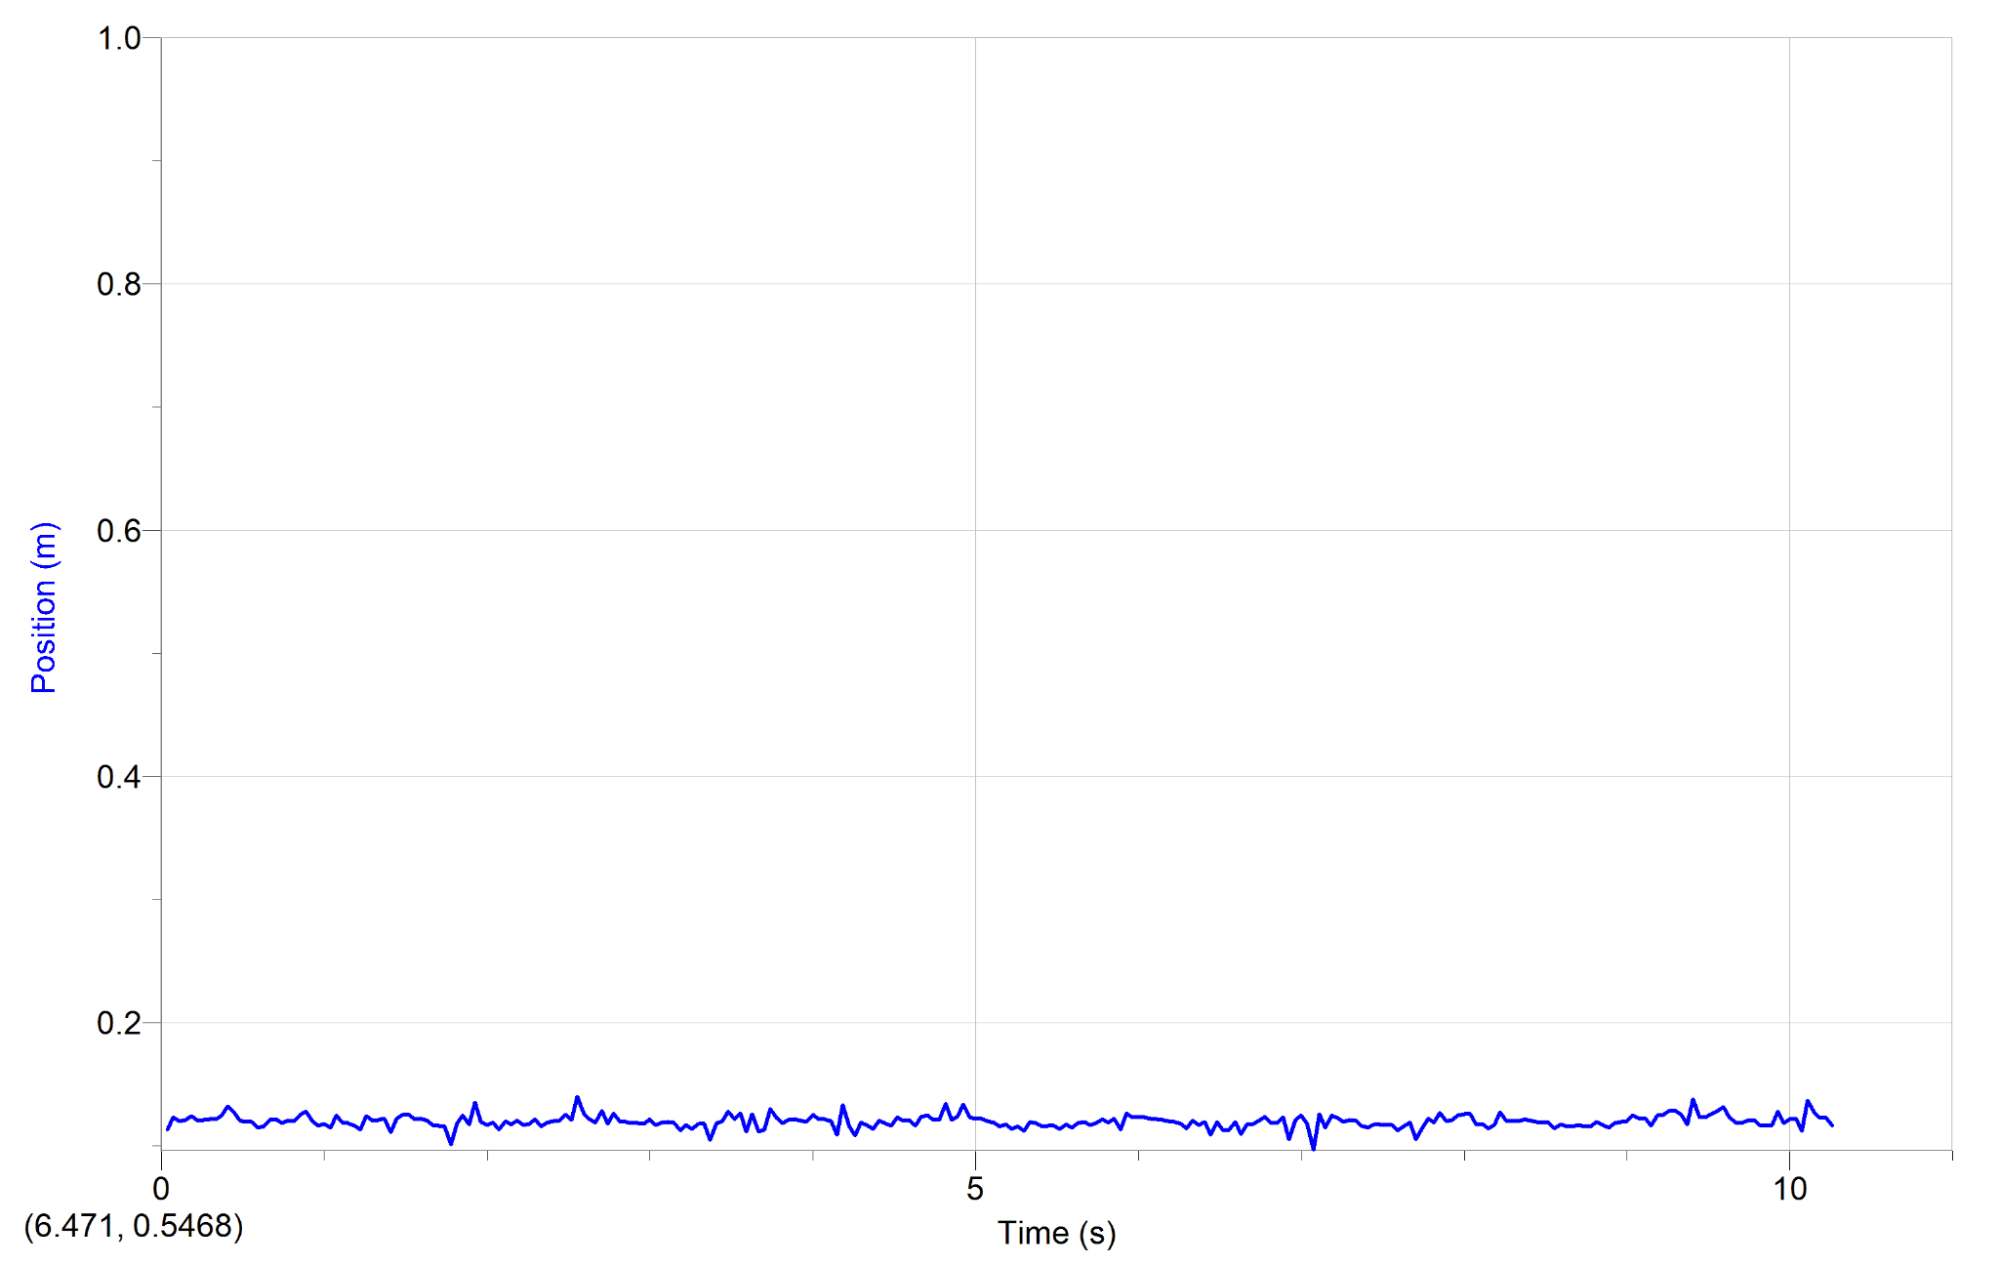
\includegraphics[width=0.5\textwidth]{image19.png}
    \end{center}

    \paragraph*{13.}

    Find the largest ``blip'', or random, sharp change in velocity, and divide that by the nearest maximum value.

    \paragraph*{14.}

    \begin{center}
        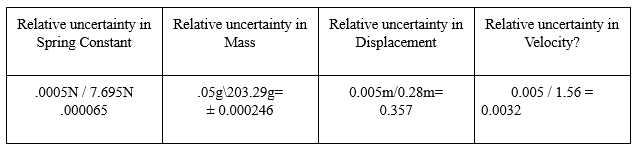
\includegraphics[width=0.9\textwidth]{images51.png}
    \end{center}

    \section*{Conclusions}

    \paragraph*{1.}

    The restoring force is in the opposite direction the spring is being stretched in. When you stretch the spring in the negative direction (compress it), the restoring force is much the same; in the opposite direction you're applying force to.

    \paragraph*{2.}

    Yes, the derivative of a sinusoidal graph is a cosinusoidal graph, meaning it's 90 degrees out of sync. Both graphs were 90 degrees out of sync with each other.

    \paragraph*{3.}

    The max amplitude of the $U$ plot was much large than the $K$ plot, however it functioned to be 90 degrees out of sync of the $K$ plot, following $E = K + U$ correctly.

    \paragraph*{4.}

    Over time they slowly lose amplitude, which is most likely cause by outside forces like friction and air resistance.

    \paragraph*{5.}

    The mechanical energy here is being leeched out of the system as stated before.

    \paragraph*{6.}

    1: Energy lost as heat via friction, 2: Energy lost to the force of air resistance, 3: energy lost to vibrations in the springs, 4: Energy lost as it's imparted into the springs and down and out of the glider.

    \paragraph*{7.}

    The $K$ recording was much lower than the $U$ recording. This is most likely due to inaccuracies in the sensor, issues in the software interpolating the points of data collected, kinetic energy being leeched from the system, and probably due to some unfamiliarity we had with the equipment and experiment. It took us about 10 minutes to figure out that rotating the motion sensor would fix the occurance of massive erroneous blips in the data.


\end{document}